\documentclass[12]{article}
\usepackage{prettyref}
\usepackage[left=2cm,right=2cm,top=2cm,bottom=2cm]{geometry}
\usepackage{graphicx}
\usepackage{amsmath, amssymb}
\usepackage{mathtools}
\usepackage{physics}
\usepackage{textcomp}
\usepackage{float}
\usepackage[british]{babel}
\usepackage{hhline}
\usepackage{multirow}
\usepackage{hyperref}
\hypersetup{
    colorlinks=true,
    linkcolor=blue,
    filecolor=magenta,      
    urlcolor=cyan,
}
\begin{document}
\begin{center}
\begin{Huge}
RESULTS-Ferromagnetic Trigger
\end{Huge}
\end{center}
%\chapter{Results}\label{ch:F}
As discussed previously, there are two trigger Hamiltonians that were studied in the course of this thesis. This chapter focuses on the performance of quantum annealing on adding the ferromagnetic trigger, $H_T^F$ to the Hamiltonian. \\
For the same transverse-field initial Hamiltonian, and each problem from the set of problem Hamiltonians (1000 12-spin SAT problems, and 91 8-spin SAT problems), ferromagnetic trigger was added to the Hamiltonian, with three different strengths, i.e. the strength parameter, g in equation (\ref{eq:n23}) was chosen to be 0.5, 1 and 2.\\
In the subsequent sections, the effect of adding the ferromagnetic trigger with different strengths will be discussed. For studying the dynamics during the evolution, same cases have been chosen as in Chapter Original Results, so that the results can be directly compared. 

\section*{g=0.5} 

On adding the ferromagnetic trigger with g= 0.5, the total instantaneous Hamiltonian becomes
\begin{equation}
H(t)=(1-s)\Big(-\sum \limits_{i=1}\limits^N h_i^x \sigma_i^x \Big)- \frac{1}{2}s(1-s)\Big( \sum \limits_{<i,j>}\sigma_{j}^x\Big) +s \Big(-\sum\limits_{i=1}\limits^{N}{h_i}^z{\sigma_i}^z - \sum\limits_{<i,j>}{J_{ij}^z} {\sigma_i}^z{\sigma_j}^z \Big).
\end{equation}
Figures (\ref{fig:f1}),(\ref{fig:f2}) and (\ref{fig:f3}) show the energy spectra for the cases 1, 2 and 3 from the previous chapter, after adding the trigger. The corresponding instantaneous energy values have also been included in these figures. 
\begin{figure}[H]
\centering 
\includegraphics[scale=0.3]{733_s12_F_g0.png}
\caption{The energy spectrum for the selected problem, with instantaneous energy values corresponding to three annealing times, with Ferromagnetic trigger, and g=0.5. $\Delta_{min}$ was found to be 0.577913, while $p$=0.999558 for $T_A$=100. }
\label{fig:f1}
\end{figure}
\begin{figure}[H]
\centering 
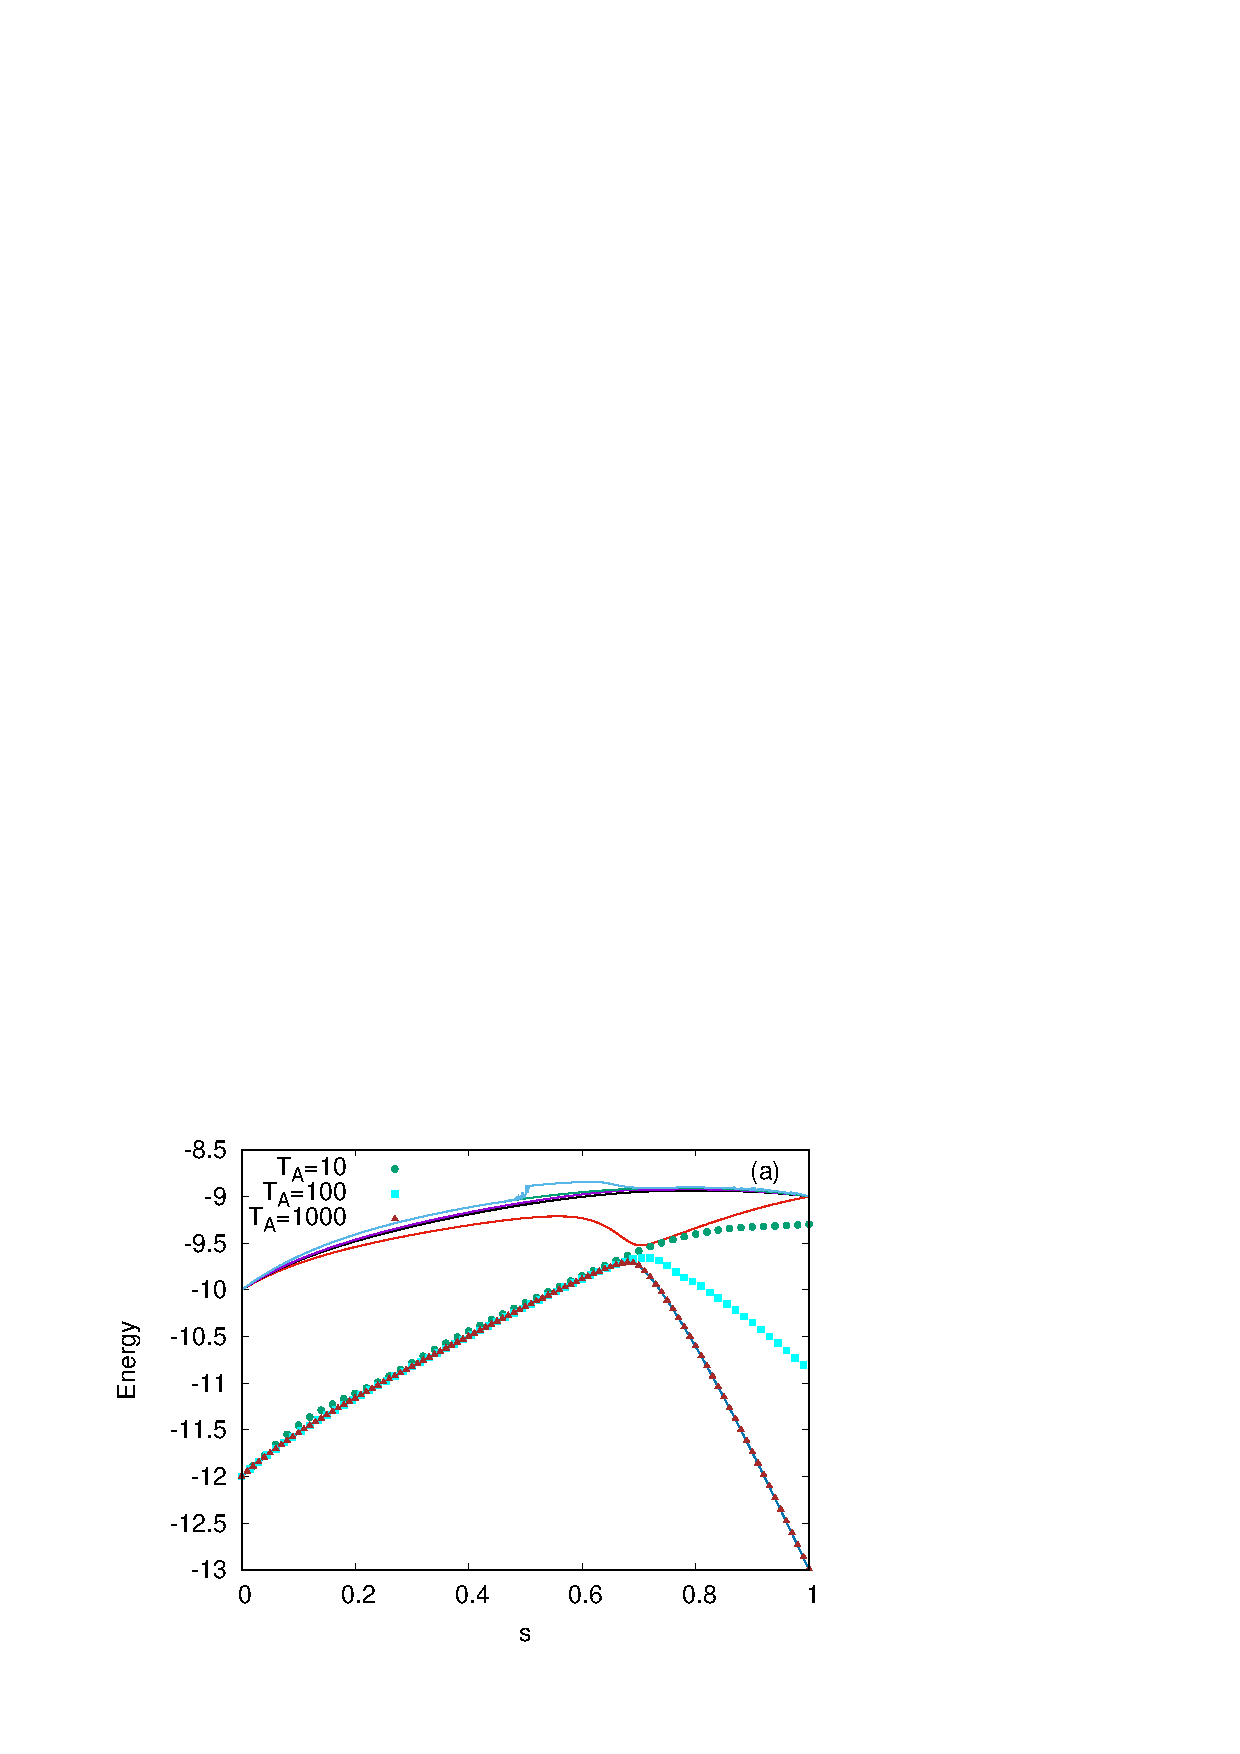
\includegraphics[scale=0.3]{950_s12_F_g0.png}
\caption{The energy spectrum for the selected problem, with instantaneous energy values corresponding to three annealing times, with Ferromagnetic trigger, and g=0.5. $\Delta_{min}$ was found to be 0.207304, while $p$=0.465049 for $T_A$=100.}
\label{fig:f2}
\end{figure}
\begin{figure}[H]
\centering 
\includegraphics[scale=0.3]{528_s12_F_g0.png}
\caption{The energy spectrum for the selected problem, with instantaneous energy values corresponding to three annealing times, with Ferromagnetic trigger, and g=0.5. $\Delta_{min}$ was found to be 0.374776, while $p$=0.957703 for $T_A$=100.}
\label{fig:f3}
\end{figure}
As a first observation, for all the three cases the minimum gap, $\Delta_{min}$ is increased as compared to the case without any triggers. This naturally increases the success probability for these cases. Table (\ref{tab:f1}) gives a comparison of the minimum gap, $\Delta_{min}$ and the ground state probability for $T_A$=100 between these values in the presence and absence of the trigger. 

\begin{table}[H]
  \centering
  \renewcommand{\arraystretch}{1.2}
  \scalebox{1.2}{%
  \begin{tabular}{|c|c|c|c|c|c|}
    \hline
    \multirow{2}{2cm}{\textbf{Case}} & \multicolumn{3}{c|}{\textbf{Minimum Gap,} $\mathbf{\Delta_{min}}$} & \multicolumn{2}{c|}{\textbf{Probability, p}}\\
    % \hline
    % \textbf{Inactive Modes} & \textbf{Description}\\
    \cline{2-6}
    & $\mathbf{\Delta_{min}^O}$ & $\mathbf{\Delta_{min}^F}$ & $\mathbf{\frac{\Delta_{min}^F}{\Delta_{min}^O}}$ & $\mathbf{p^O}$ & $\mathbf{p^F}$\\
    %\hhline{~--}
    \hline
    1 & 0.440730 & 0.577913 & 1.31126 & 0.994433 & 0.999558 \\ \hline
    2 & 0.031213 & 0.207374 & 6.64383 & 0.014638 & 0.465049 \\ \hline
    3 & 0.157325 & 0.374776 & 2.98074 & 0.519862 & 0.957703  \\ \hline
  \end{tabular}}
  \caption{A comparison of the minimum gap and the success probability at $T_A$=100 for the chosen cases, in the absence (represented with a superscript O for Original) and presence (represented with a superscript F for Ferromagnetic) trigger, with strength g=0.5. In all the chosen cases the gaps increase upon adding the ferromagnetic trigger, thereby improving the success probability.}
  \label{tab:f1}
\end{table}
In the absence of any triggers, the success probability in the second case was quite small for $T_A$=100. Upon adding the ferromagnetic trigger, this probability improves significantly, or more precisely, by a  factor of 31.8 (see figures (\ref{fig:o3}) and (\ref{fig:f2}) for reference). Moreover, for the third case, there is also some improvement in the success probability, by a factor of 1.8 (compare figures (\ref{fig:o4}) and (\ref{fig:f3})), owing to the increase in the minimum energy gap. \\

Similarly, the success probabilities were evaluated for all the problems in the set, for the annealing times $T_A \in {10,100,1000}$. The resulting success probabilities were then compared to the case without any triggers, and the ratio of the two success probabilities has been referred to as the relative success probability in this work. Figures (\ref{fig:f4}),(\ref{fig:f5}) and (\ref{fig:f6}) show the histogram for the distribution of the relative success probability for $T_A \in \{0.5,1,2\}$ respectively.
\begin{figure}[H]
\centering 
\includegraphics[scale=0.3]{Hist_s12_T10_F_g0.png}
\caption{The distribution of relative success probability=$\frac{p^F}{p^O}$ for $T_A$=10, where $p^O$ is the success probability of the Hamiltonian without adding any trigger, and $p^F$ is the success probability after adding Ferromagnetic trigger to the Hamiltonian.}
\label{fig:f4}
\end{figure}
For $T_A$=10, the success probabilities for all the cases upon adding the ferromagnetic trigger, is greater than the success probability of the original Hamiltonian. The mean relative success probability is 3.041, while the mode of the distribution is 1.995. The range of the relative success probability is from 1.259 to 562.341. 
\begin{figure}[H]
\centering 
\includegraphics[scale=0.3]{Hist_s12_T100_F_g0.png}
\caption{The distribution of relative success probability=$\frac{p^F}{p^O}$ for $T_A$=100, where $p^O$ is the success probability of the Hamiltonian without adding any trigger, and $p^F$ is the success probability after adding Ferromagnetic trigger to the Hamiltonian.}
\label{fig:f5}
\end{figure}
For $T_A$=100, the success probability is either improved or remains unchanged, on adding the ferromagnetic trigger, for all the cases. For this case, the average relative success probability is 3.531, and 3.548 is the mode for the distribution. However, the range of the relative success probability shrinks from 1 to 31.622.
\begin{figure}[H]
\centering 
\includegraphics[scale=0.3]{Hist_s12_T1000_F_g0.png}
\caption{The distribution of relative success probability=$\frac{p^F}{p^O}$ for $T_A$=1000, where $p^O$ is the success probability of the Hamiltonian without adding any trigger, and $p^F$ is the success probability after adding Ferromagnetic trigger to the Hamiltonian.}
\label{fig:f6}
\end{figure}
As for $T_A$=100, for $T_A$=1000 as well, the relative success probability either increases or remains unchanged as result of adding the ferromagnetic trigger. The spread of relative success probability decreases to the range of 1 to 6.309. The mean value for the distribution is 1.170, while the mode is equal to 1. \\

An important point to be noted is the significance of decreasing values of relative success probability on increasing annealing times. For a given problem (fixed minimum gap), the overlap between the final state and the ground state of the problem should increase with increasing the annealing time, if the evolution is adiabatic. Therefore, if a given annealing time is long enough for the system state to always stay close to the instantaneous ground state with the original Hamiltonian (without triggers), there is not too much scope of improvement by adding the ferromagnetic trigger. The decreasing relative success probability values are thus suggestive of an improvement in the success probability of the original Hamiltonian upon increasing annealing times.\\

Figure (\ref{fig:f7}) shows the scatter plot of the the success probabilities of all the problems upon adding the ferromagnetic trigger against the original success probability for the corresponding problem. Such a plot is helpful in understanding the difficulty of the problem (in terms of its success probability) before and after adding the trigger.
\begin{figure}[H]
\centering 
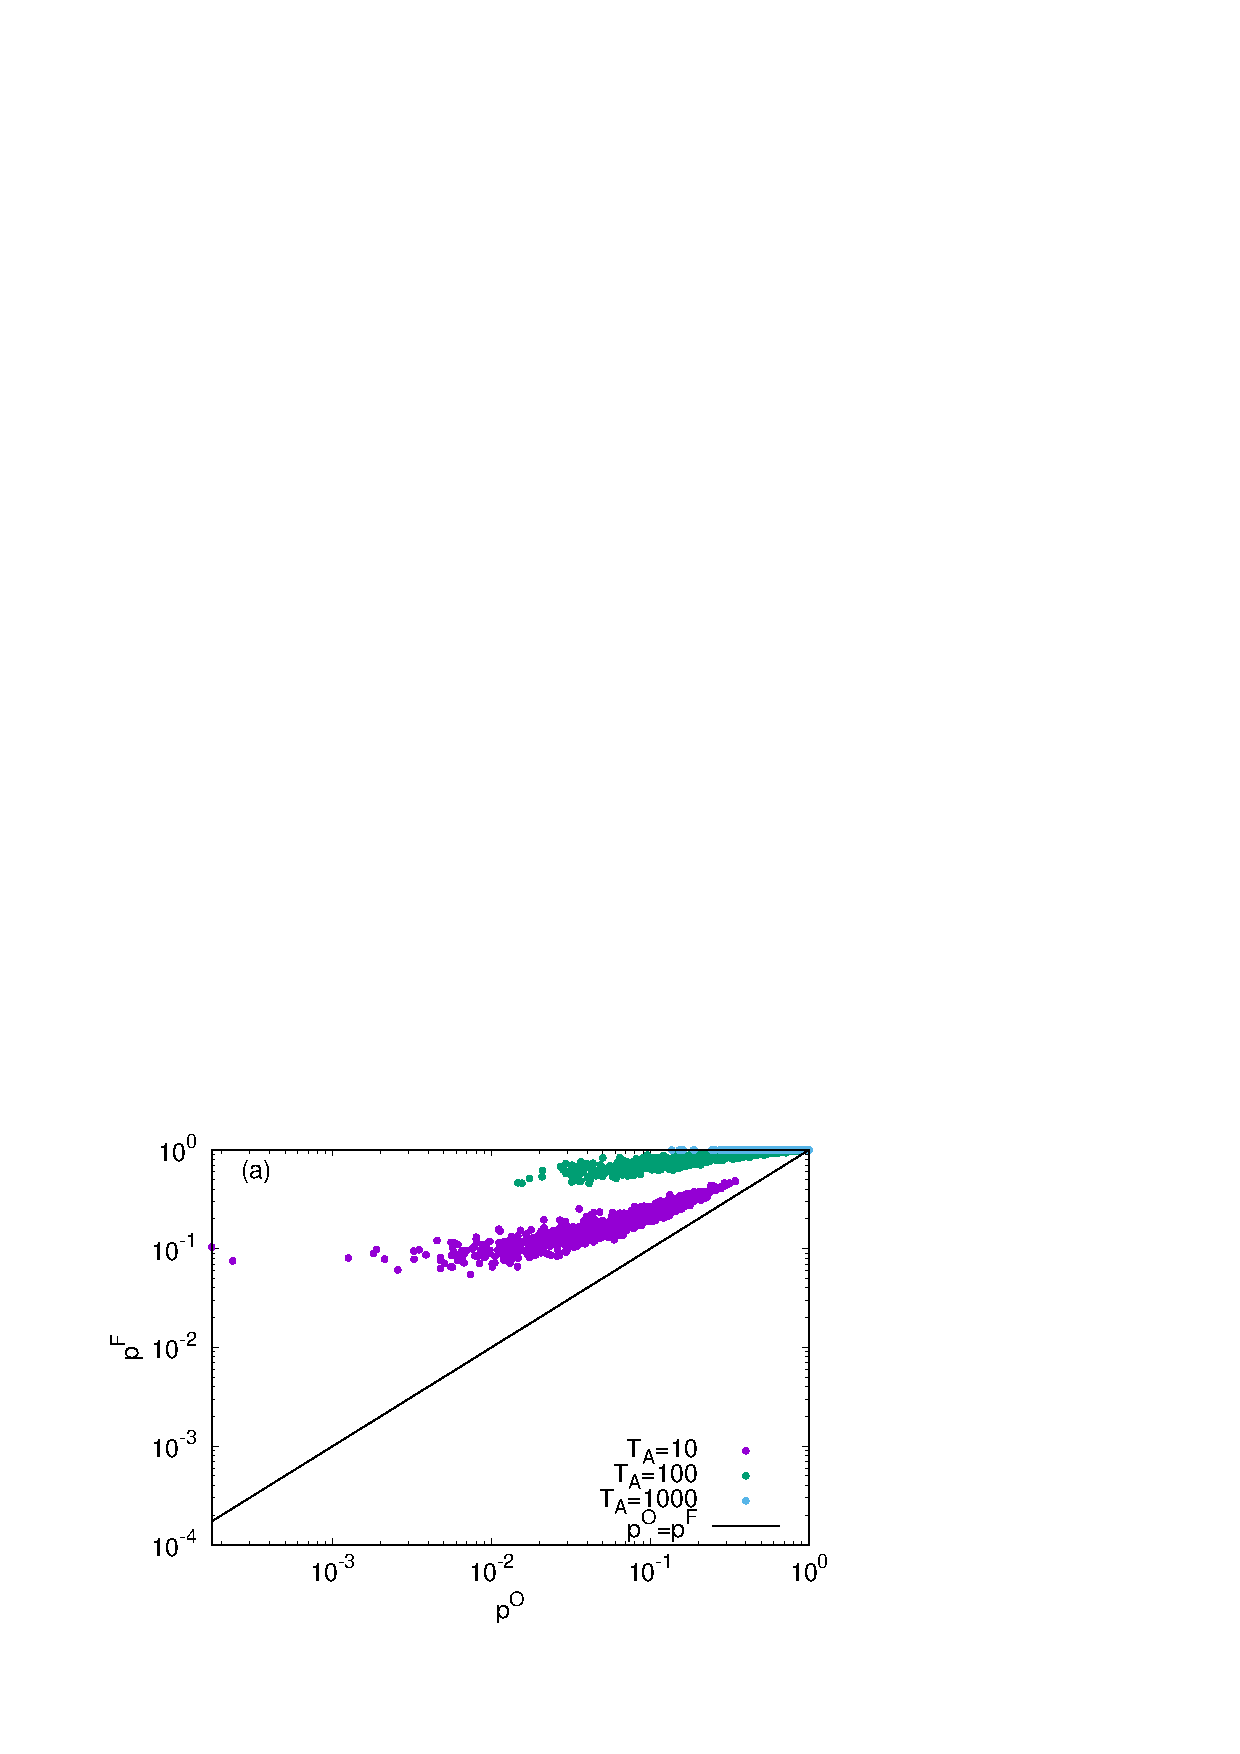
\includegraphics[scale=0.3]{Scatt_s12_F_g0.png}
\caption{Scatter plot for the success probability with ferromagnetic trigger against the success probability with the original Hamiltonian, for annealing time $T_A \in \{0.5,1,2\}$. The line represents the cases where the success probability remains unchanged.}
\label{fig:f7}
\end{figure}
As expected, for $T_A$=1000, all the problems of the set already have a large success probability with the original Hamiltonian. Therefore these cases lie close to the the line $p^O=p^F$. Since for $T_A$=10, the initial ground state probabilities are not as high, the ferromagnetic trigger can significantly increase the success probability. The range of the affected problems is therefore larger in this case. The spread for $T_A$=100 lies between the other two cases.

\section*{g=1}
A similar analysis was done with the strength parameter set to 1. The instantaneous Hamiltonian then becomes:
\begin{equation}
H(t)=(1-s)\Big(-\sum \limits_{i=1}\limits^N h_i^x \sigma_i^x \Big)- s(1-s)\Big( \sum \limits_{<i,j>}\sigma_{j}^x\Big) +s \Big(-\sum\limits_{i=1}\limits^{N}{h_i}^z{\sigma_i}^z - \sum\limits_{<i,j>}{J_{ij}^z} {\sigma_i}^z{\sigma_j}^z \Big).
\end{equation}
Figures (\ref{fig:f8} \ref{fig:f9} \ref{fig:f10}) show the energy spectra for the three cases chosen in the last chapter upon adding the Ferromagnetic trigger with g=1. 
\begin{figure}[H]
\centering 
\includegraphics[scale=0.3]{733_s12_F_g1.png}
\caption{The energy spectrum for the selected problem, with instantaneous energy values corresponding to three annealing times, with Ferromagnetic trigger, and g=1. $\Delta_{min}$ was found to be 0.69084, while $p$=0.99981 for $T_A$=100. }
\label{fig:f8}
\end{figure}
\begin{figure}[H]
\centering 
\includegraphics[scale=0.3]{950_s12_F_g1.png}
\caption{The energy spectrum for the selected problem, with instantaneous energy values corresponding to three annealing times, with Ferromagnetic trigger, and g=1. $\Delta_{min}$ was found to be 0.41289, while $p$=0.88895 for $T_A$=100.}
\label{fig:f9}
\end{figure}
\begin{figure}[H]
\centering 
\includegraphics[scale=0.3]{528_s12_F_g1.png}
\caption{The energy spectrum for the selected problem, with instantaneous energy values corresponding to three annealing times, with Ferromagnetic trigger, and g=1. $\Delta_{min}$ was found to be 0.54389, while $p$=0.99454 for $T_A$=100.}
\label{fig:f10}
\end{figure}
The minimum gaps in all the chosen cases, were found to have increased, not only in comparison to the case without triggers, but also compared to the case with g=0.5. Table (\ref{tab:f2}) shows a contrast between the minimum energy values and the success probability between the original Hamiltonian and the Hamiltonian in the presence of ferromagnetic trigger with g=1. 

\begin{table}[H]
  \centering
  \renewcommand{\arraystretch}{1.2}
  \scalebox{1.2}{%
  \begin{tabular}{|c|c|c|c|c|c|}
    \hline
    \multirow{2}{2cm}{\textbf{Case}} & \multicolumn{3}{c|}{\textbf{Minimum Gap,} $\mathbf{\Delta_{min}}$} & \multicolumn{2}{c|}{\textbf{Probability, p}}\\
    % \hline
    % \textbf{Inactive Modes} & \textbf{Description}\\
    \cline{2-6}
    & $\mathbf{\Delta_{min}^O}$ & $\mathbf{\Delta_{min}^F}$ & $\mathbf{\frac{\Delta_{min}^F}{\Delta_{min}^O}}$ & $\mathbf{p^O}$ & $\mathbf{p^F}$\\
    %\hhline{~--}
    \hline
    1 & 0.44073 & 0.69084 & 1.56749 & 0.99443 & 0.99981 \\ \hline
    2 & 0.03121 & 0.41289 & 13.22941 & 0.01463 & 0.88895 \\ \hline
    3 & 0.15732 & 0.54389 & 3.45722 & 0.51986 & 0.99454  \\ \hline
  \end{tabular}}
  \caption{A comparison of the minimum gap and the success probability at $T_A$=100 for the chosen cases, in the absence (represented with a superscript O for Original) and presence (represented with a superscript F for Ferromagnetic) trigger, with strength g=1. In all the chosen cases the gaps increase upon adding the ferromagnetic trigger, thereby improving the success probability.}
  \label{tab:f2}
\end{table}

\begin{figure}[H]
\centering 
\includegraphics[scale=0.3]{Hist_s12_T10_g1.png}
\caption{The distribution of relative success probability=$\frac{p^F}{p^O}$ for $T_A$=10, where $p^O$ is the success probability of the Hamiltonian without adding any trigger, and $p^F$ is the success probability after adding Ferromagnetic trigger to the Hamiltonian.}
\label{fig:f4}
\end{figure}
For $T_A$=10, the success probabilities for all the cases upon adding the ferromagnetic trigger, is greater than the success probability of the original Hamiltonian. The mean relative success probability is 6.251, while the mode of the distribution is 3.981. The range of the relative success probability is from 1.412 to 1778.279. 

\begin{figure}[H]
\centering 
\includegraphics[scale=0.3]{Hist_s12_T100_g1.png}
\caption{The distribution of relative success probability=$\frac{p^F}{p^O}$ for $T_A$=100, where $p^O$ is the success probability of the Hamiltonian without adding any trigger, and $p^F$ is the success probability after adding Ferromagnetic trigger to the Hamiltonian.}
\label{fig:f5}
\end{figure}
For $T_A$=100, the success probability is either improved or remains unchanged, on adding the ferromagnetic trigger, for all the cases. For this case, the average relative success probability is 4.365, and 4.467 and 6.309 are the modes for the distribution. However, the range of the relative success probability shrinks from 1 to 63.096.
\begin{figure}[H]
\centering 
\includegraphics[scale=0.3]{Hist_s12_T1000_g1.png}
\caption{The distribution of relative success probability=$\frac{p^F}{p^O}$ for $T_A$=1000, where $p^O$ is the success probability of the Hamiltonian without adding any trigger, and $p^F$ is the success probability after adding Ferromagnetic trigger to the Hamiltonian.}
\label{fig:f6}
\end{figure}
As for $T_A$=100, for $T_A$=1000 as well, the relative success probability either increases or remains unchanged as result of adding the ferromagnetic trigger. The spread of relative success probability decreases to the range of 1 to 6.456. The mean value for the distribution is 1.237, while the mode is equal to 1. \\
\section*{g=2}
\begin{figure}[H]
\centering 
\includegraphics[scale=0.3]{Hist_s12_T10_g2.png}
\caption{The distribution of relative success probability=$\frac{p^F}{p^O}$ for $T_A$=10, where $p^O$ is the success probability of the Hamiltonian without adding any trigger, and $p^F$ is the success probability after adding Ferromagnetic trigger to the Hamiltonian.}
\label{fig:f4}
\end{figure}
For $T_A$=10, the success probabilities for all the cases upon adding the ferromagnetic trigger, is greater than the success probability of the original Hamiltonian. The mean relative success probability is 6.251, while the mode of the distribution is 3.981. The range of the relative success probability is from 1.412 to 1778.279. 

\begin{figure}[H]
\centering 
\includegraphics[scale=0.3]{Hist_s12_T100_g2.png}
\caption{The distribution of relative success probability=$\frac{p^F}{p^O}$ for $T_A$=100, where $p^O$ is the success probability of the Hamiltonian without adding any trigger, and $p^F$ is the success probability after adding Ferromagnetic trigger to the Hamiltonian.}
\label{fig:f5}
\end{figure}
For $T_A$=100, the success probability is either improved or remains unchanged, on adding the ferromagnetic trigger, for all the cases. For this case, the average relative success probability is 4.365, and 4.467 and 6.309 are the modes for the distribution. However, the range of the relative success probability shrinks from 1 to 63.096.
\begin{figure}[H]
\centering 
\includegraphics[scale=0.3]{Hist_s12_T1000_g2.png}
\caption{The distribution of relative success probability=$\frac{p^F}{p^O}$ for $T_A$=1000, where $p^O$ is the success probability of the Hamiltonian without adding any trigger, and $p^F$ is the success probability after adding Ferromagnetic trigger to the Hamiltonian.}
\label{fig:f6}
\end{figure}
As for $T_A$=100, for $T_A$=1000 as well, the relative success probability either increases or remains unchanged as result of adding the ferromagnetic trigger. The spread of relative success probability decreases to the range of 1 to 6.456. The mean value for the distribution is 1.237, while the mode is equal to 1. \\
\end{document}